\chapter{Resultados e Discussão}\label{cap:resultados}

\section{Detecção e Reconhecimento}
\subsection{ICDAR 2011}\label{sec:results_icdar_2011}
O conjunto de imagens de validação do ICDAR 2011 conta com 141 imagens e é importante constatar o fato que são imagens de 
relativa baixa resolução para os padrões atuais, onde as maiores contêm cerca de 315 mil píxeis. São caracterizadas por 
estarem no contexto de imagens de anúncios e anexos de e-mails, com textos primariamente horizontais.

Ao aplicar a solução sobre os exemplos de validação da base de dados, em desempenho, todas as imagens foram processadas com 
sucesso em 36,31 segundos em um ambiente com aceleração gráfica, média de 257 milissegundos por imagem. Para fins comparativos, 
a mesma tarefa agora executada sem a aceleração gráfica levou 328,44 segundos, cerca de 9 vezes mais tempo, executando na 
mesma máquina alocada no serviço Paperspace, que consta com 30 GB de memória RAM, disponibilidade de processamento gráfico 
com NVIDIA QUADRO M4000 e processamento CPU baseado em instâncias AWS C4, disponibilizam 8 núcleos, 16 \textit{threads} do 
processador Intel Xeon E5-2666, com frequência de operação em 2,9 GHz.

Apesar do maior tempo de processamento, o uso da solução em ambientes sem uma placa gráfica compatível ainda não se torna 
inviável, sobretudo considerando que a média de tempo de processamento por imagem foi de 2,32 segundos. No entanto, fica 
desencorajado a execução sobre um conjunto muito grande de imagens, já que o processamento corresponde a uma carga muito 
alta dependendo do \textit{hardware} onde a solução for executada, visto que a execução em CPU alocou 17,4 GB de memória, 
volume maior do que a quantidade total de grande parte dos sistemas mais domésticos.

Para executar o \textit{script} de avaliação dos resultados da solução, o comando abaixo pode ser executado, fornecendo o 
caminho para um arquivo comprimido que contém os resultados para cada imagem do conjunto de validação.

\begin{minted}{bash}
            python script.py –g=gt.zip –s=res_img_.zip
\end{minted}

O resultado da melhor configuração foi o apresentado na Tabela \ref{tab:icdar11_results}. Em suma, a avaliação usa três 
métricas: precisão, \textit{recall} e F1-Score. A Precisão é a relação dos acertos (verdadeiros positivos) sobre a contagem 
total de predições positivas (verdadeiros positivos e falsos positivos), ou seja, dentre as predições da solução, qual 
é a porcentagem de acerto. O \textit{recall} relaciona a quantidade de acertos com a quantidade total de casos verdadeiros. 
O F1-Score é basicamente a média harmônica das métricas precisão e \textit{recall}.

\begin{minted}{bash}
                Calculated!
                {
                    "precision": 0.7068273092369478,
                    "recall": 0.7343532684283728,
                    "hmean": 0.7203274215552524, 
                    "AP": 0
                }
\end{minted}

\begin{table}[htb]
    \centering
    \caption{Avaliação de resultados sobre a base ICDAR 2011.}
    \begin{tabular}{|c|c|c|}
        \hline
        Precisão (\%) & Recall (\%) & F1-Score (\%) \\
        \hline
        70,68 & 73,44 & 72,03\\
        \hline
    \end{tabular}
    \label{tab:icdar11_results}
\end{table}

Em resumo, isso demonstra que a cada 100 palavras detectadas e processadas, aproximadamente 70 tiveram o texto corretamente 
extraído. É um resultado satisfatório para o trabalho desenvolvido e o nível de simplicidade adotado. Estes números colocariam 
essa solução em nono lugar entre 18 outros trabalhos submetidos na plataforma de desafios \textit{Robust Reading Competition}.

\begin{figure}
    \centering
    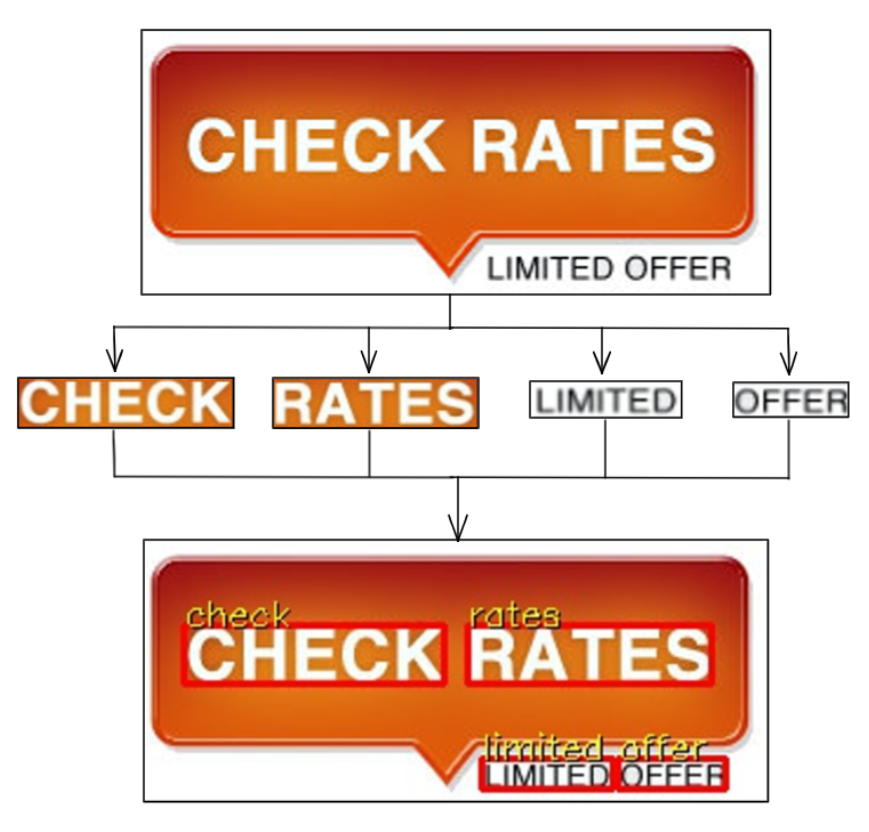
\includegraphics[width=0.5\textwidth]{figs/resultados-icdar11-01.png}
    \caption{Exemplo de resultado de reconhecimento. Imagem 52 do conjunto de validação.}
    \label{fig:results_icdar11_01}
\end{figure}

A Figura \ref{fig:results_icdar11_01} exemplifica as etapas da solução apresentada. A imagem de entrada é processada pela rede de 
detecção que extrai as regiões de texto regredindo as coordenadas das \textit{bounding-boxes}. Com isso, essas regiões são então 
cortadas da imagem original e alimentam a rede de reconhecimento para extração do texto decodificado.

Apesar do resultado satisfatório, o mais interessante é aprofundar não nos acertos, onde o modelo reconheceu as palavras certas, 
mas sim onde ele errou e identificar limitações e, eventualmente, futuras otimizações.

Um dos casos mais evidentes onde a solução apresentou problemas foi na presença de caracteres especiais. Uma das limitações do 
modelo de reconhecimento é a lista de caracteres passíveis de reconhecimento, que contempla apenas os caracteres do alfabeto da 
língua inglesa, de A até Z, adicionado dos dígitos decimais, de 0 até 9. Este dicionário limitado restringe muito a capacidade 
de detecção em que não são tão difíceis de observar. Caracteres de pontuação, acentos, marcações como o cifrão (\$), entre 
outros casos, acabam dificultando o acerto do reconhecimento. A Figura \ref{fig:results_icdar11_02} exemplifica esta constatação. 
Nela, é possível observar que o trecho que representa o preço do artigo anunciado na imagem 5 do conjunto de validação, que 
contém cifrão, vírgula e asterisco, não foi reconhecida com sucesso. Apesar de o método aproximar bem os caracteres desconhecidos, 
reconhecendo o cifrão (\$) como um cinco (5) e o asterisco (*) como a letra X, o resultado não é satisfatório nesse caso.

\begin{figure}
    \centering
    
\includegraphics[width=0.75\textwidth]{figs/resultados-icdar11-02.png}
    \caption{Comparação entre entrada e saída sobre a imagem 5 do conjunto de validação do ICDAR 2011}
    \label{fig:results_icdar11_02}
\end{figure}

Outra dificuldade ficou aparente em imagens de baixa resolução, que acabam contendo regiões de texto ainda menores. Em geral, 
a regressão das \textit{bounding-boxes} fica um pouco mais grosseira, mas ainda satisfatórias. Entretanto, a maior limitação 
foi o reconhecimento. As regiões de texto recortadas da imagem original acabam ficando bem pequenas e com pouca definição, o 
que trouxe dificuldades para o modelo pré-treinado CRNN utilizado. A Figura \ref{fig:results_icdar11_03} exemplifica essa 
dificuldade. Pode-se observar que nenhum dos “títulos” de cada uma das fotos que estão presentes na Figura \ref{fig:results_icdar11_03} 
foram localizadas com sucesso, mas não obtiveram a igualdade entre predição e gabarito (ficaram marcadas com uma área azul).

\begin{figure}
    \centering
    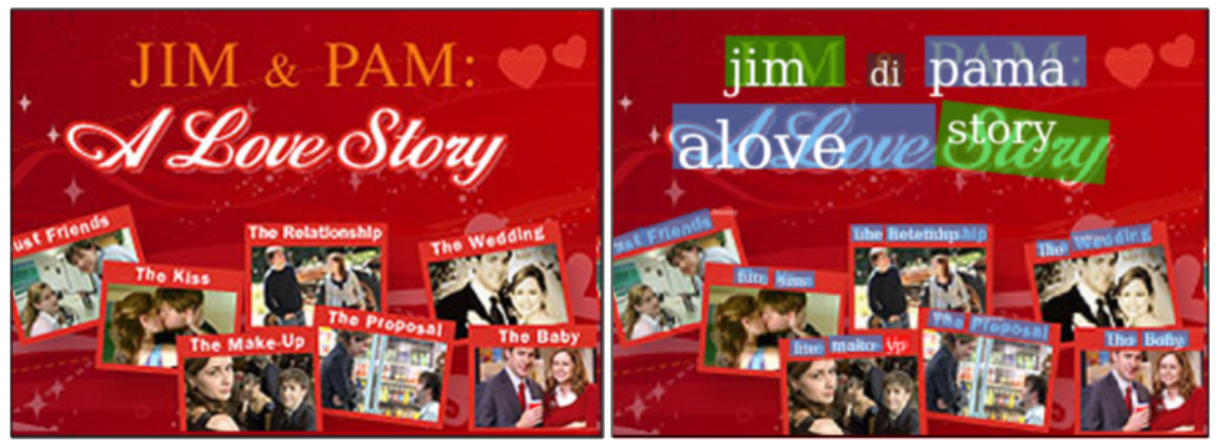
\includegraphics[width=0.75\textwidth]{figs/resultados-icdar11-03.png}
    \caption{Exemplo de imagem com instâncias de texto bem pequenas em resolução. Imagem 28 do ICDAR 2011}
    \label{fig:results_icdar11_03}
\end{figure}

Outro detalhe que demonstra uma dificuldade mais global do problema de reconhecimento de texto em cenas é a fonte utilizada 
na frase “A Love Story”, na região superior da Figura \ref{fig:results_icdar11_03}. Apesar de o reconhecimento ter relativo 
sucesso nesse exemplo, a localização não conseguiu segmentar corretamente todas as palavras da frase. A generalização da detecção 
e do reconhecimento para as mais diversas categorias de fontes é um dos principais problemas que motivam o uso de redes neurais 
profundas para reconhecimento de texto. [\citeonline{StrDlEra}]

O ICDAR 2011 apresenta casos mais complexos de detecção de reconhecimento de texto se comparado ao contexto de aplicações OCR 
convencionais, que lidam com reconhecimento de texto estruturado, sem grandes variações de fontes e planos de fundo, o que é 
bastante válido para avaliar a solução. No entanto, ainda não são casos reais de texto em cena, problema que motivou este trabalho. 
A base de dados ICDAR 2013 contém exemplos mais característicos de texto de cena.

%%%%%%%%%%%%%%%%%%%%%%%%%%%%%%%%%%%%%%%%%%%%%%%%%%%%%%%%%%%%%%%%%%%%%%%%%%%%%%%%%%%%%%%%%%%%%%%%%%%%%%%%%%%%%%%%%%%%%%%%%%%%%%%%%%%%%%%%%%%%%%%%%%%%%%%%%%%%%%%%%%

\subsection{ICDAR 2013}\label{sec:results_icdar_2013}

O conjunto de imagens de validação do ICDAR 2013 conta com 233 imagens de tamanhos variados. As menores têm cerca de 640 píxeis 
de altura e 480 píxeis de comprimento, enquanto as maiores têm dimensões comparáveis à resolução 4K, com 3888 píxeis de altura e 
2592 píxeis de comprimento. Vale ressaltar que as imagens passam por uma redução em resolução ao entrarem no modelo CRAFT, que 
maximiza a maior dimensão da imagem para 1280 píxeis e ajusta a segunda dimensão mantendo a relação de aspecto original, justamente 
para otimizar o desempenho do método.

Ao aplicar a solução sobre os exemplos de validação da base de dados, em desempenho, todas as imagens foram processadas com sucesso 
em 207,74 segundos em um ambiente com aceleração gráfica, utilizando os mesmos recursos computacionais disponíveis na validação do 
ICDAR 2011, atingindo uma média de 892 milissegundos por imagem. A média de tempo de processamento por imagem é 3,5 vezes maior 
quando comparado à base de dado anterior, ICDAR 2011.  As predições não foram executadas sem aceleração gráfica por economia de 
recursos.

Com base nas mesmas métricas apresentadas na Seção \ref{sec:results_icdar_2011}, durante a discussão sobre os resultados contra 
o ICDAR 2011, a avaliação da solução no ICDAR 2013 demonstra resultados similares aos vistos na Seção \ref{sec:results_icdar_2011}, 
disponíveis na Tabela \ref{tab:icdar13_results}. Cerca de 7 acertos a cada 10 predições. Tendo em vista que é uma base um pouco 
mais desafiadora, é um resultado novamente satisfatório. Comparando precisão e \textit{recall}, nota-se um desvio maior, cerca 
de 6 pontos percentuais, indicando mais falsos positivos, ou seja, regiões detectadas como regiões de texto que não estão nas 
anotações de gabarito. Em alguns casos, uma mesma palavra acabou sendo segmentada de maneira errada, em outros, regiões visivelmente 
de não-texto foram detectadas. A Figura \ref{fig:results_icdar13_01} demonstra esse fenômeno.

\begin{minted}{bash}
                Calculated!
                {
                    "precision": 0.7043390514631686,
                    "recall": 0.7611777535441657,
                    "hmean": 0.7316561844863733, 
                    "AP": 0
                }
\end{minted}

\begin{table}[htb]
    \centering
    \caption{Avaliação de resultados sobre a base ICDAR 2013.}
    \begin{tabular}{|c|c|c|}
        \hline
        Precisão (\%) & Recall (\%) & F1-Score (\%) \\
        \hline
        70,43 & 76,11 & 73,17\\
        \hline
    \end{tabular}
    \label{tab:icdar13_results}
\end{table}

\begin{figure}
    \centering
    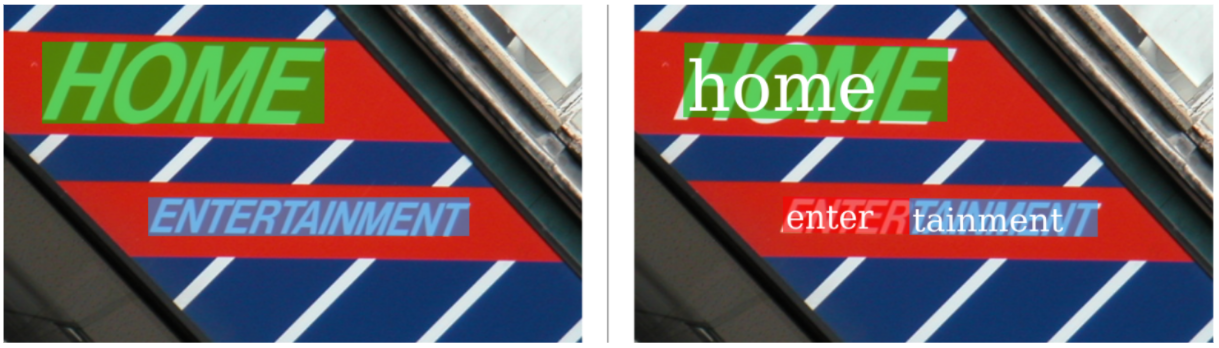
\includegraphics[width=0.75\textwidth]{figs/resultados-icdar13-01.png}
    \caption{Demonstração de um falso positivo durante a avaliação da solução contra a base de dados ICDAR 2013.}
    \label{fig:results_icdar13_01}
\end{figure}

Entretanto, as principais dificuldades de detecção e reconhecimento são compartilhadas com o que foi observado durante a avaliação 
na base ICDAR 2011. Caracteres especiais, pontuação e acentos são limitações conhecidas do reconhecimento.

Por introduzir mais exemplos de imagens verdadeiramente com textos em ambientes naturais, algumas novas dificuldades apareceram. 
O desafio que provavelmente é mais evidente está relacionado aos eventuais artefatos nas imagens decorrentes de reflexos em 
algumas imagens de texto sob vidro ou com incidência de iluminação de alta intensidade (\textit{flashes} de câmeras fotográficas), 
onde, em alguns exemplos, a detecção foi sub-ótima (Figura \ref{fig:results_icdar13_03}) e em outros, o reconhecimento não foi 
o melhor (Figura \ref{fig:results_icdar13_02}).

\begin{figure}
    \centering
    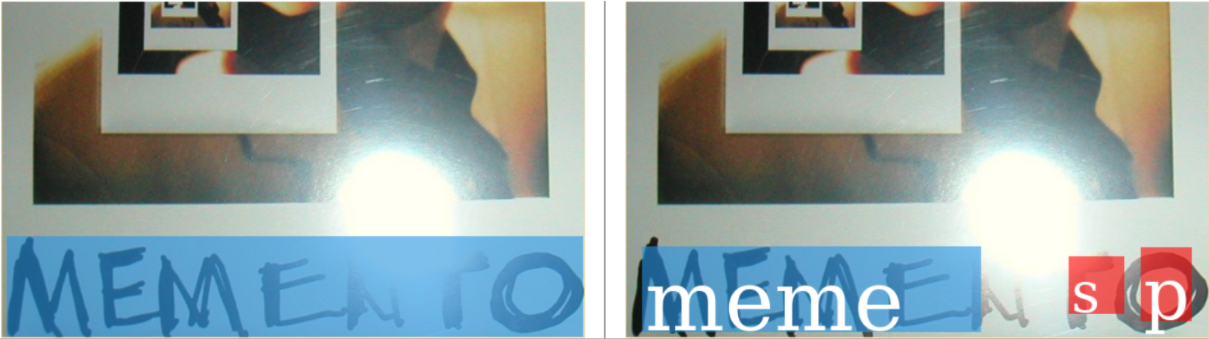
\includegraphics[width=0.75\textwidth]{figs/resultados-icdar13-03.png}
    \caption{Exemplo de imagem com artefatos que trouxeram dificuldades para a localização correta do texto.}
    \label{fig:results_icdar13_03}
\end{figure}

\begin{figure}
    \centering
    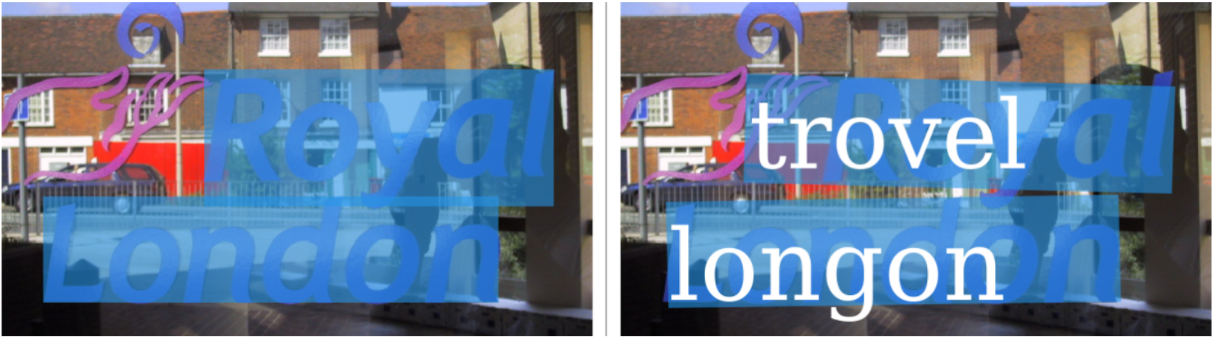
\includegraphics[width=0.75\textwidth]{figs/resultados-icdar13-02.png}
    \caption{Exemplo de texto sob vidro, com plano de fundo desafiadores para o reconhecimento.}
    \label{fig:results_icdar13_02}
\end{figure}

Outra dificuldade conhecida de problemas de reconhecimento de texto em cenas está relacionada a palavras em destaque, o que pode 
ser relativamente comum, dado o contexto de uma imagem com diversos objetos na cena. Apesar de ser um exemplo mais simples, a 
Figura \ref{fig:results_icdar13_04} demonstra esse caso. A etiqueta na infusão está visivelmente em desfoque e complicou o 
trabalho do reconhecimento por deixar os caracteres mais ambíguos.

\begin{figure}
    \centering
    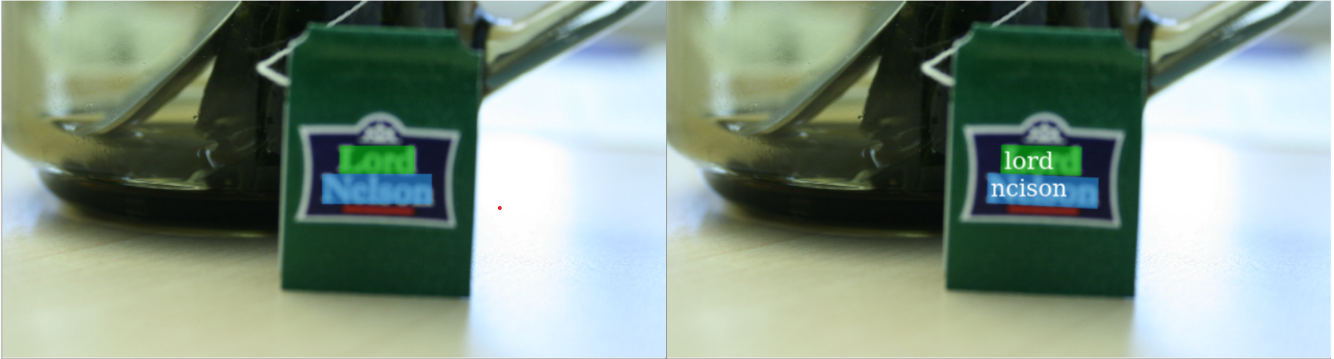
\includegraphics[width=\textwidth]{figs/resultados-icdar13-04.png}
    \caption{Exemplo de imagem com texto em desfoque.}
    \label{fig:results_icdar13_04}
\end{figure}

%%%%%%%%%%%%%%%%%%%%%%%%%%%%%%%%%%%%%%%%%%%%%%%%%%%%%%%%%%%%%%%%%%%%%%%%%%%%%%%%%%%%%%%%%%%%%%%%%%%%%%%%%%%%%%%%%%%%%%%%%%%%%%%%%%%%%%%%

\subsection{Imagens autorais}\label{sec:results_own_images}
Com caráter mais qualitativo, é interessante inferir a qualidade das soluções em imagens fora do contexto das bases de dados 
conhecidamente utilizadas para treino e validação, para experienciar a qualidade do reconhecimento em imagens do dia-a-dia. 
Com esse objetivo, algumas imagens no álbum pessoal do autor deste trabalho foram selecionadas para passarem pela solução 
apresentada. Alguns exemplos estão disponíveis abaixo.

\begin{figure}
    \centering
    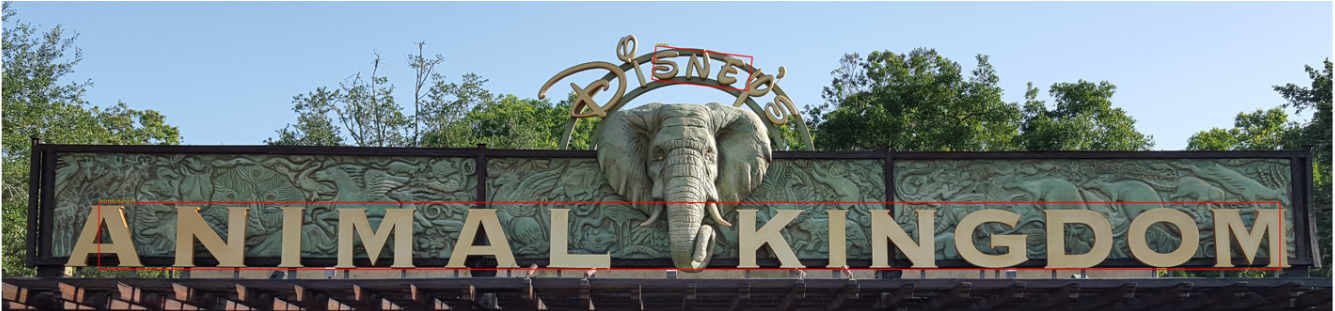
\includegraphics[width=\textwidth]{figs/resultados-autoral-01.png}
    \caption{Exemplo de imagem autoral onde a solução apresentou dificuldades com texto curvo e estilizado. Textos reconhecidos: “sney” e “intmalakingon”.}
    \label{fig:results_own_images_01}
\end{figure}

\begin{figure}
    \centering
    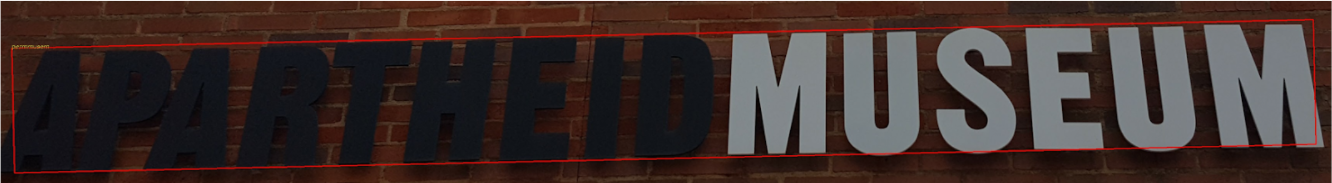
\includegraphics[width=\textwidth]{figs/resultados-autoral-02.png}
    \caption{Exemplo de imagem autoral onde uma região de texto muito longa não foi extraída muito bem, principalmente no início 
    da palavra, o que dificultou o reconhecimento. Texto reconhecido: “permmusem”.}
    \label{fig:results_own_images_02}
\end{figure}

Algumas imagens utilizadas foram bastante desafiadoras para a solução, tanto em localização quanto em reconhecimento. Imagens 
com texto bem localizado e visível, alguns letreiros e placas tiveram bons resultados, mas alguns casos de palavras mais longas 
e curvadas, mesmo que levemente, não tiveram muito sucesso, especialmente se apresentarem caligrafia muito estilizadas, como é 
possível observar na Figura \ref{fig:results_own_images_03}. A respeito de textos curvados, melhorias na solução poderiam 
melhorar a situação, como a aplicação de soluções para transformar as imagens antes de passar pelo reconhecimento como, por 
exemplo, uma rede STN (\textit{Spatial Transformer Network} [\citeonline{STN}]), de modo a obter uma imagem com o mínimo de 
curvatura possível, facilitando o trabalho de reconhecimento.

\begin{figure}
    \centering
    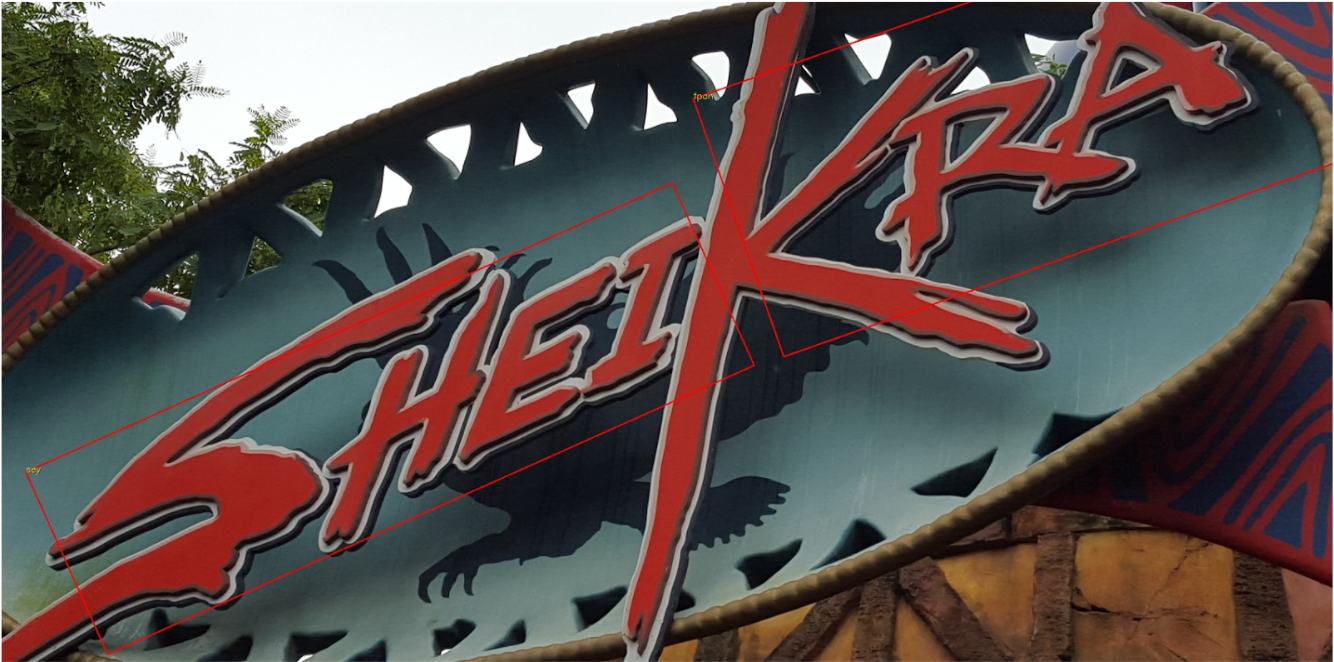
\includegraphics[width=0.7\textwidth]{figs/resultados-autoral-03.png}
    \caption{Exemplo de imagem autoral com fontes bastante estilizadas que trouxeram dificuldade tanto para a detecção, quanto 
    para o reconhecimento. Textos reconhecidos: “sey” e “fpan”.}
    \label{fig:results_own_images_03}
\end{figure}


Um exemplo foi bastante interessante, pois contrariou as expectativas quanto ao reconhecimento, demonstrando o potencial que a 
solução pode apresentar com algumas iterações de melhorias. A Figura \ref{fig:results_own_images_04} mostra um caso de sucesso 
na localização e reconhecimento onde o contexto onde o texto está inserido tem bastante informação e a fonte do texto, 
principalmente do trecho escrito “Disney’s”, é bastante estilizado, e mesmo assim, o reconhecimento foi bem preciso.


Agora, quando o texto se encontra em situações bastante favoráveis, por exemplo, bem iluminado, sem oclusões, em geral, disposto 
horizontalmente e com caligrafia não rebuscada, a solução atinge o seu potencial máximo, conseguindo localizar e interpretar 
com muita precisão. A Figura \ref{fig:results_own_images_05} demonstra esse caso, onde temos um cartaz de boas-vindas do 
museu do Apartheid, na África do Sul.

\begin{figure}
    \centering
    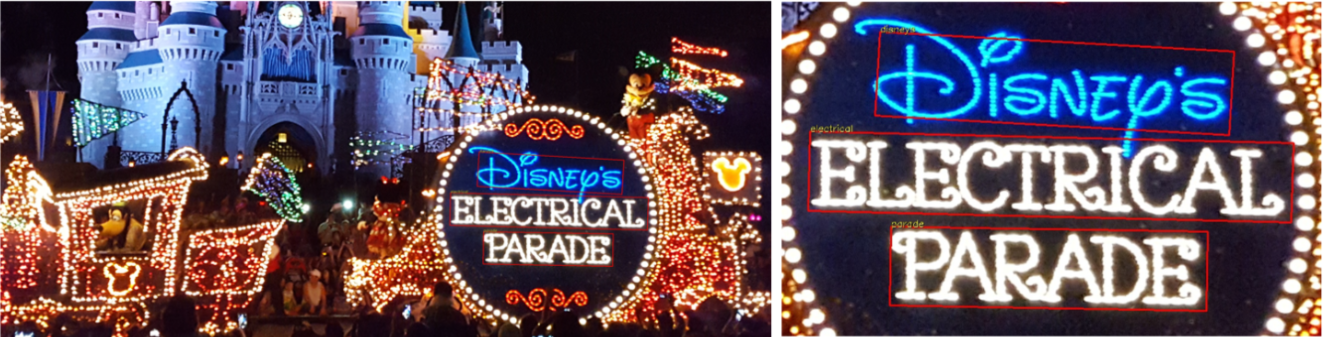
\includegraphics[width=\textwidth]{figs/resultados-autoral-04.png}
    \caption{Exemplo de reconhecimento com sucesso em condições desafiadoras em imagem autoral. Textos reconhecidos: “disneys”, 
    "electrical" e “parade”.}
    \label{fig:results_own_images_04}
\end{figure}

\begin{figure}
    \centering
    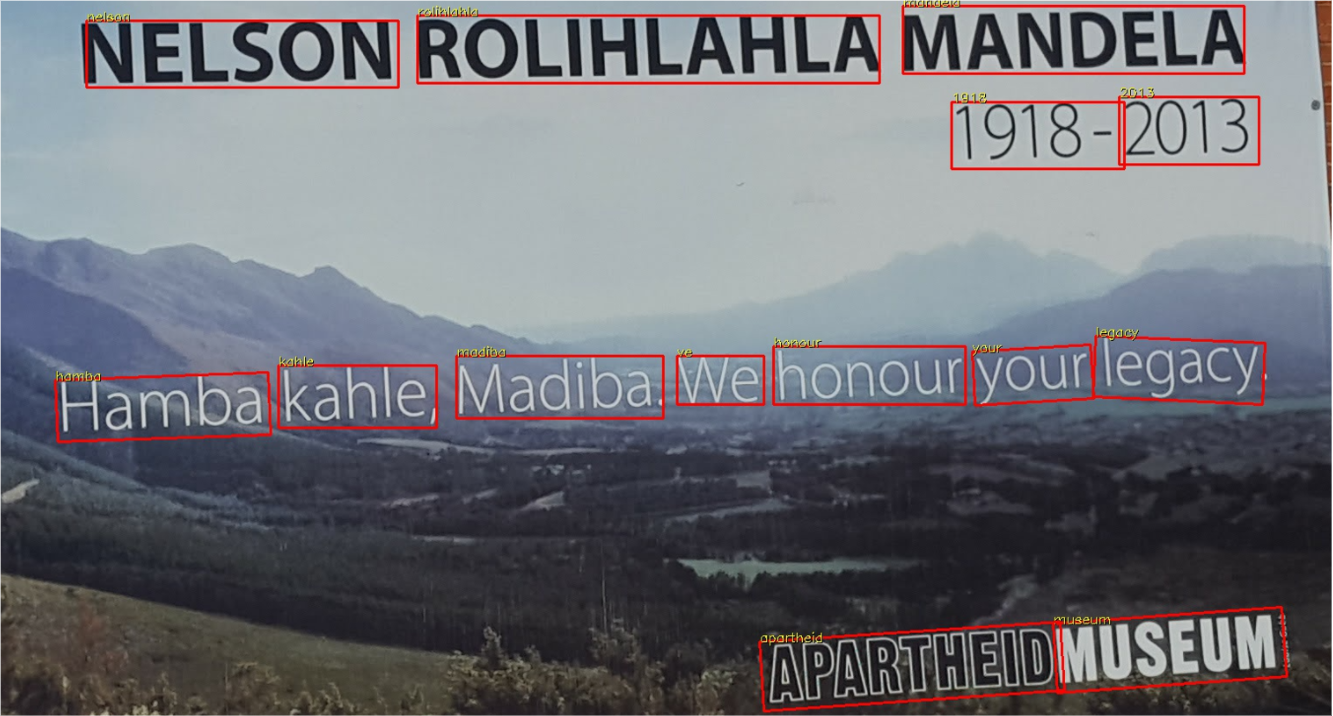
\includegraphics[width=0.75\textwidth]{figs/resultados-autoral-05.png}
    \caption{Exemplo de imagem autoral com alta precisão de reconhecimento. Textos reconhecidos: “nelson”, “rolihlahla” “mandela”, 
    “1918”, “2013”, “hamba”, “kahle”, “madiba”, “ve”, “honour”, “your”, “legacy”, “apartheid”, “museum”.}
    \label{fig:results_own_images_05}
\end{figure}


\section{Disponibilização em nuvem}
O resultado da prova de conceito de publicar a aplicação final em um ambiente remoto através de computação em nuvem foi de relativo 
sucesso. Ao final de todas as etapas citadas em \ref{sec:methodology_cloud_deploy}, a aplicação foi publicada na plataforma do 
Heroku com sucesso. No entanto, como constatado na Seção \ref{sec:results_icdar_2011}, a demanda de recursos computacionais da 
solução integrada foi é relativamente grande, em especial a pressão sobre disponibilidade de memória RAM no sistema é grande.

O ambiente disponibilizado de graça pelo Heroku é bastante limitado em recursos, por questões óbvias, portanto já não era esperado 
um bom desempenho, sobretudo pelo fato do ambiente não contar com aceleração gráfica.

A partir de alguns testes sobre aplicação publicada, pode-se observar que o ambiente não é de fato estável para a aplicação publicada. 
Ao requisitar a execução do reconhecimento em imagens menores da base de dados ICDAR 2011, com dimensões próximas de 300px por 300px 
ainda é possível obter uma resposta do servidor, porém para imagens maiores e mais pesadas, a aplicação ultrapassa os limites de 
memória que tem disponível para o contêiner e, como medida de segurança imposta pelo Heroku, o contêiner é desligado sem conseguir 
terminar o processo de reconhecimento.
